


\section{Effect of \moe Sparsity on Downstream Task Performance}
\label{sec:scaling_law_ds}
In this section, we study how sparsity affects the relationship between upstream and downstream performance of \moes. In other words, does sparsity impact the relative gains from improvements in pretraining tasks on downstream tasks?

We use downstream tasks from the evaluation suite in~\texttt{llm-foundry}\footnote{Github repository: \url{https://github.com/mosaicml/llm-foundry}} for benchmarking our pretrained models, specifically in an in-context few-shot learning setup. This setup focuses on evaluating a model's ability to learn and adapt to new tasks with limited examples.
The downstream task are devided into four pre-defined categories namely: language understanding, world knowledge, reading comprehension, and symbolic reasoning to help us systematically test whether the downstream vs upstream performance trend remains the same or is different as we vary sparsity values.

\begin{figure*}[!t]
    \centering
    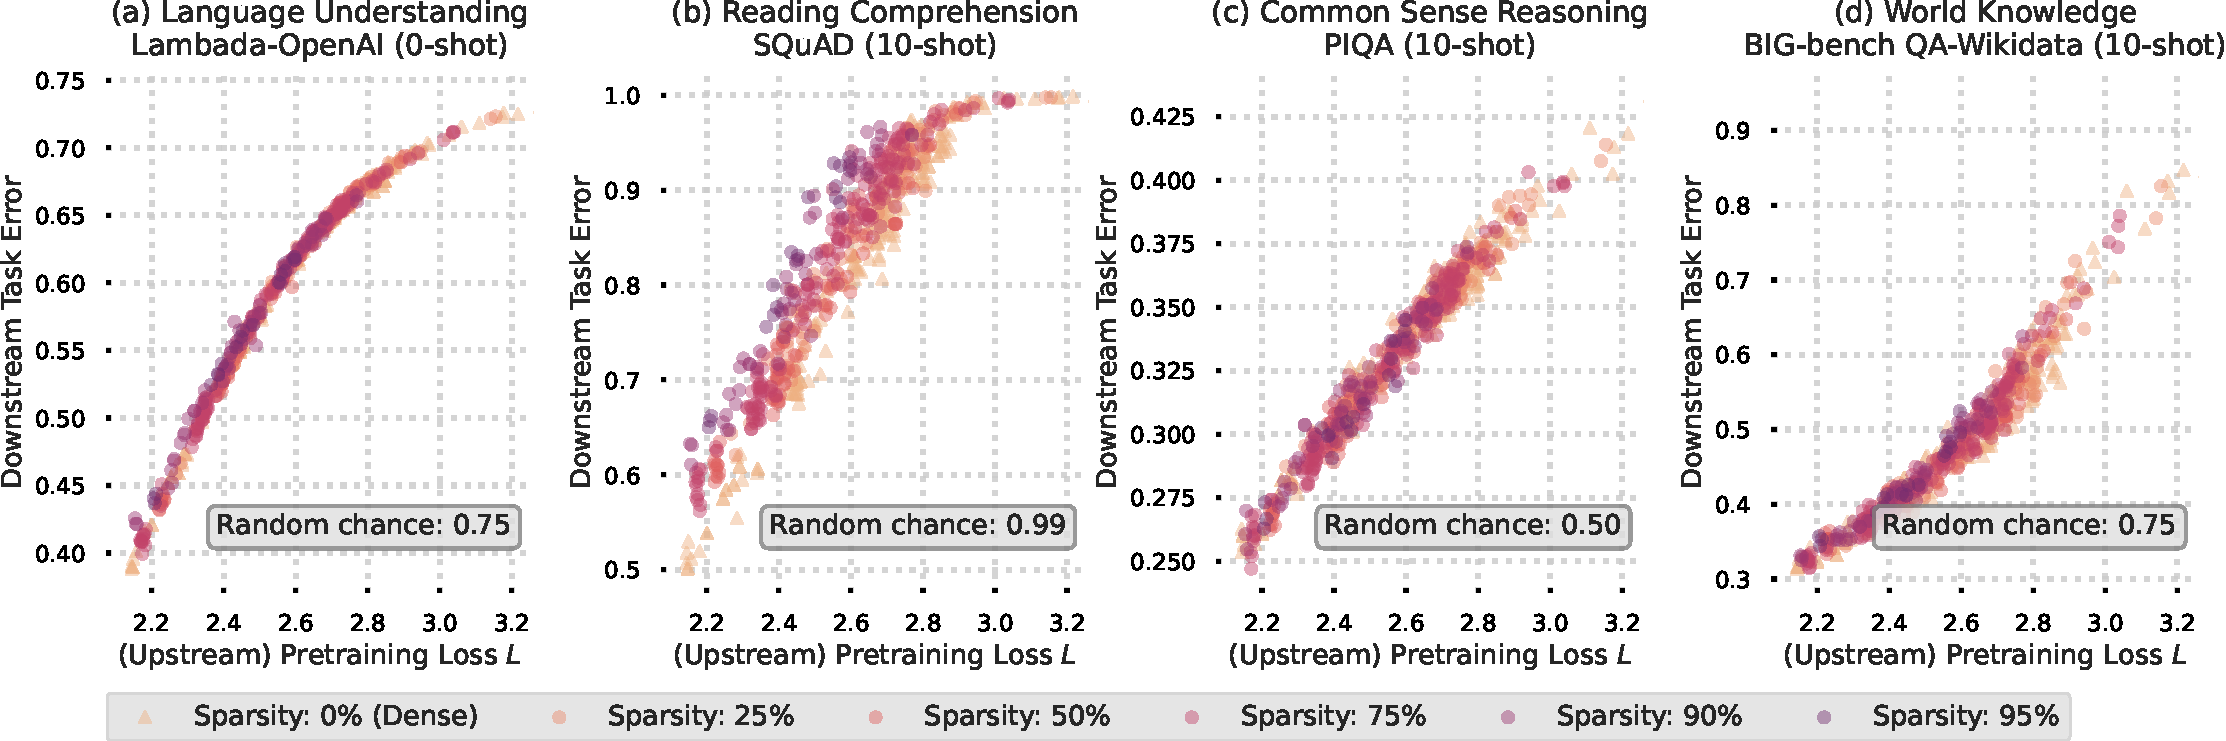
\includegraphics[width=0.95\textwidth]{plots/s4_plot.pdf}
    \caption{
    \textbf{Effect of sparsity on downstream vs upstream performance.} Downstream error shows a tight relationship with pretraining (``upstream'') loss across downstream tasks across all sparsity levels. 
    }
    \label{fig:downstream}
\vspace{-15pt}
\end{figure*}

We observe from ~\Cref{fig:downstream}a (language understanding), ~\Cref{fig:downstream}c (commonsense reasoning), and ~\Cref{fig:downstream}d (world knowledge) that, in an in-context few-shot learning setting, there is a strong correlation between upstream (pretraining) loss and downstream performance (error) across all these tasks. For these tasks, downstream performance in the few-shot setting is predictable based on upstream performance, regardless of the sparsity level. This indicates that, in the context of these tasks, the optimal sparsity level follows the same trend as the optimal sparsity observed during pretraining.
%Furthermore, \moes downstream performance improve with increasing sparsity levels. 
However,~\Cref{fig:downstream}b (reading comprehension) shows an example of a task where models with higher sparsity transfer more poorly compared to denser models. This decrease in the transfer performance of sparser models on these tasks may be due to the lower inference-time compute in sparser models compared to their denser counterparts for a similar pretraining loss. Further analysis is needed to verify this intuition. 

If fewer \flops per example are the reason behind the worse transfer performance in sparser models, this effect might diminish with a larger total training compute budget, as the optimal active number of parameters increases. Moreover, one can use approaches like chain-of-thought reasoning~\citep{wei2022chain_cot} to independently increase \flops per example during inference time. 

In \Cref{app:cot_expt}, we explore whether increasing inference-time compute via Chain-of-Thought (CoT) prompting can improve the performance of MoEs on tasks that require more reasoning. Our experiments indicate that MoEs benefit more from this increased compute compared to dense models with a similar number of active parameters. This suggests that dynamic compute allocation during inference may be crucial for MoEs to perform well on complex reasoning tasks.

While our results may indicate that there may be no additional benefit obtained via sparsity in \moes beyond the efficiency gains for pretraining, we caution the reader that this suggestion may be an artifact of the scale of our experiments. In the end, since, as shown in \S\ref{sec:n_s_d_interaction}, sparser models are more efficient both in terms of training and inference cost (when measured in terms of theoretical \flops), we can reach better pretraining performance with higher sparsity levels at a lower cost, which can translate to better downstream performance.

% Better pretraining performance can be achieved with increased sparsity without sacrificing either training or inference cost (when measured in terms of theoretical \flops).

% We observe that for tasks in the categories of language understanding, an example of which is shown in~\Cref{fig:s4}a, and world knowledge, ~\Cref{fig:s4}d, there is a tight relationship between upstream and downstream performance, i.e., a model with a low pretraining loss also has a low downstream error. Furthermore, models performance improve with sparsity.

% Interestingly, for tasks that fall into the reading comprehension category, an example of which is shown in~\Cref{fig:s4}b, sparsity seem to have a negative effect, i.e., given two models with the same pretraining loss, a denser model is more likely to have a lower downstream error.  
% Intuitively, a reason behind this could be that denser models use more compute during inference as they have higher number of active parameters. This suggests that methods like chain of thought reasoning could potentially help close the gap as we increase the sparsity level of models. We defer further investigation of this hypothesis to future work.

% TODO complete the following
% These results suggest that \moes with higher sparsity levels show improved performance over their lower sparsity counterparts. However, the results do not suggest that \moes unlock additional capability in the downstream tasks considered in our work

% These results suggest, there is no significant additional benefit when introducing sparsity in \moes for transfer, at the current scale of our experiments. Since, as shown in section~\ref{}, sparser models are more efficient both in terms of training and inference cost (when measured in terms of theoretical \flops), we can reach a better pretraining performance with sparser models at a lower cost. Hence, sparser models are generally more favorable. \todo[inline]{need a better way to phrase this.}

% To further confirm this, in Figure~\ref{}, we show how DS performance changes as a function active number of parameters (proxy for inference cost) and training compute budget. We observe that ...
% \todo[inline]{what exactly do we want to plot to summerize the message}.

% Previous studies have shown ...


% Scaling law for predicting DS loss fiven US loss (perplexity on the pretraining data), when architecture and pretraining data are fixed:
% \begin{equation}
% L(DS) = k \cdot L(US)^{\alpha} + e
% \label{eq:ds_us_scaling}
% \end{equation}

% First, we fit this equation for dense models as well as models with different sparsity levels. We investigate weather the sparsity level impact the scaling law co-efficents for predicting DS perfomrance from US performance. 
